\documentclass[aspectratio=169,10pt]{beamer}

% =========================================================
% Modern Foundation Models -- Lecture 1
% Stanford/CME295-inspired visual style, original HIT template
% =========================================================

\usepackage[utf8]{inputenc}
\usepackage[T1]{fontenc}
\usepackage{lmodern}
\usepackage{amsmath,amssymb}
\usepackage{tikz}
\usepackage{booktabs}
\usepackage{array}
\usepackage{graphicx}
\usepackage{xcolor}
\usepackage{hyperref}
\usetikzlibrary{arrows.meta,positioning,calc,shapes.geometric,fit,decorations.pathreplacing}

% ---------- Colors ----------
\definecolor{hitred}{RGB}{145,20,20}
\definecolor{softred}{RGB}{230,95,95}
\definecolor{textdark}{RGB}{35,45,50}
\definecolor{lightgray}{RGB}{236,236,236}
\definecolor{fadegray}{RGB}{205,205,205}
\definecolor{boxblue}{RGB}{205,222,247}
\definecolor{boxgreen}{RGB}{213,236,207}
\definecolor{boxpink}{RGB}{244,204,204}
\definecolor{boxorange}{RGB}{255,229,199}
\definecolor{boxpurple}{RGB}{221,213,239}

% ---------- Beamer cleanup ----------
\setbeamertemplate{navigation symbols}{}
\setbeamertemplate{headline}{}
\setbeamertemplate{footline}{}
\setbeamercolor{normal text}{fg=textdark,bg=white}
\setbeamerfont{frametitle}{size=\Large,series=\mdseries}

% ---------- Layout constants ----------
\newcommand{\TopBarHeight}{0.72}
\newcommand{\SlideFooter}{%
  \begin{tikzpicture}[remember picture,overlay]
    \node[anchor=south west,font=\scriptsize\bfseries,text=textdark] at ([xshift=0.12cm,yshift=0.10cm]current page.south west) {Holon Institute of Technology};
    \node[anchor=south east,font=\scriptsize\bfseries,text=hitred] at ([xshift=-0.14cm,yshift=0.10cm]current page.south east) {HIT};
  \end{tikzpicture}%
}

\newcommand{\SlideTitle}[1]{%
  \begin{tikzpicture}[remember picture,overlay]
    \fill[hitred] (current page.north west) rectangle ([yshift=-0.72cm]current page.north east);
    \node[anchor=west,font=\fontsize{22}{26}\selectfont,text=white] at ([xshift=0.55cm,yshift=-0.36cm]current page.north west) {#1};
  \end{tikzpicture}%
  \vspace*{0.58cm}%
  \SlideFooter%
}

\newenvironment{hitframe}[1]{%
  \begin{frame}[plain]
  \SlideTitle{#1}
}{%
  \end{frame}
}

% ---------- Helpers ----------
\newcommand{\hlred}[1]{\textcolor{softred}{#1}}
\newcommand{\faded}[1]{\textcolor{fadegray}{#1}}
\newcommand{\source}[1]{%
  \begin{tikzpicture}[remember picture,overlay]
    \node[anchor=south west,font=\tiny\itshape,text=softred] at ([xshift=1.9cm,yshift=0.10cm]current page.south west) {#1};
  \end{tikzpicture}%
}

\newcommand{\token}[3][]{\node[draw=#2, fill=white, rounded corners=0.5pt, inner xsep=7pt, inner ysep=5pt, font=\ttfamily\small,#1]{#3};}
\newcommand{\modelbox}[2][]{\node[draw=textdark, fill=boxblue, minimum width=1.0cm, minimum height=0.56cm, font=\small,#1]{#2};}

% ---------- Section overview slide ----------
\newcommand{\CourseOverview}[1]{%
\begin{frame}[plain]
\begin{tikzpicture}[remember picture,overlay]
  \fill[white] (current page.south west) rectangle (current page.north east);
  \fill[hitred] ([xshift=0.52\paperwidth]current page.south west) rectangle (current page.north east);
  \node[anchor=center,font=\fontsize{25}{31}\selectfont\bfseries,text=textdark,align=center] at ([xshift=-0.24\paperwidth,yshift=0.25cm]current page.center) {Modern\\Foundation\\Models};
  \node[anchor=south west,font=\scriptsize\bfseries,text=textdark] at ([xshift=0.12cm,yshift=0.10cm]current page.south west) {Holon Institute of Technology};
  \node[anchor=south east,font=\scriptsize\bfseries,text=hitred] at ([xshift=-0.14cm,yshift=0.10cm]current page.south east) {HIT};
  \node[anchor=west,align=left,font=\fontsize{17}{23}\selectfont,text=white] at ([xshift=0.56\paperwidth,yshift=2.3cm]current page.center) {\ifnum#1=1\bfseries\fi NLP overview};
  \node[anchor=west,align=left,font=\fontsize{17}{23}\selectfont,text=white!65!gray] at ([xshift=0.56\paperwidth,yshift=1.55cm]current page.center) {\ifnum#1=2\color{white}\bfseries\fi Tokenization};
  \node[anchor=west,align=left,font=\fontsize{17}{23}\selectfont,text=white!65!gray] at ([xshift=0.56\paperwidth,yshift=0.80cm]current page.center) {\ifnum#1=3\color{white}\bfseries\fi Word representation};
  \node[anchor=west,align=left,font=\fontsize{17}{23}\selectfont,text=white!65!gray] at ([xshift=0.56\paperwidth,yshift=0.05cm]current page.center) {\ifnum#1=4\color{white}\bfseries\fi RNNs};
  \node[anchor=west,align=left,font=\fontsize{17}{23}\selectfont,text=white!65!gray] at ([xshift=0.56\paperwidth,yshift=-0.70cm]current page.center) {\ifnum#1=5\color{white}\bfseries\fi Self-attention mechanism};
  \node[anchor=west,align=left,font=\fontsize{17}{23}\selectfont,text=white!65!gray] at ([xshift=0.56\paperwidth,yshift=-1.45cm]current page.center) {\ifnum#1=6\color{white}\bfseries\fi Transformer architecture};
  \node[anchor=west,align=left,font=\fontsize{17}{23}\selectfont,text=white!65!gray] at ([xshift=0.56\paperwidth,yshift=-2.20cm]current page.center) {\ifnum#1=7\color{white}\bfseries\fi End-to-end example};
  \draw[white!70!gray,line width=1.5pt] ([xshift=0.56\paperwidth,yshift=-2.75cm]current page.center) -- ++(0.8,0);
\end{tikzpicture}
\end{frame}%
}

\title{Modern Foundation Models}
\subtitle{Lecture 1: From NLP to Transformers}
\author{Dror Lederman}
\institute{Holon Institute of Technology}
\date{\today}

\begin{document}

% ---------------------------------------------------------
% Title slide
% ---------------------------------------------------------
\begin{frame}[plain]
\begin{tikzpicture}[remember picture,overlay]
  \fill[white] (current page.south west) rectangle (current page.north east);
  \node[anchor=north west,fill=hitred,text=white,font=\Large,minimum width=2.0cm,minimum height=0.55cm] at (current page.north west) {Lecture 1};
  \node[anchor=north,align=center,font=\fontsize{26}{32}\selectfont\bfseries,text=hitred] at ([yshift=-0.42cm]current page.north) {Modern Foundation Models\\[-1mm] \& Large Language Models};
  \draw[hitred,line width=2pt] ([xshift=2.2cm,yshift=-2.1cm]current page.north west) -- ([xshift=-2.2cm,yshift=-2.1cm]current page.north east);
  \node[anchor=center,align=center,font=\fontsize{18}{22}\selectfont\bfseries,text=hitred] at ([yshift=-2.15cm]current page.center) {Lecture 1: From NLP to Transformers};
  \node[anchor=center,align=center,font=\fontsize{14}{18}\selectfont,text=textdark] at ([yshift=-3.1cm]current page.center) {Dror Lederman};
  \node[anchor=south west,font=\scriptsize\bfseries,text=textdark] at ([xshift=0.12cm,yshift=0.10cm]current page.south west) {Holon Institute of Technology};
  \node[anchor=south east,font=\scriptsize\bfseries,text=hitred] at ([xshift=-0.14cm,yshift=0.10cm]current page.south east) {HIT};
\end{tikzpicture}
\end{frame}

% ---------------------------------------------------------
\begin{hitframe}{Welcome!}
\vspace{0.45cm}
{\Large \textbf{Goals.}}
\vspace{0.35cm}
\begin{enumerate}
  \setlength\itemsep{0.35cm}
  \item Understand how \textbf{Transformers} work and how they relate to \textbf{LLMs}
  \item Learn how \textbf{LLMs are trained} and used in modern applications
  \item Build the background needed for \textbf{foundation models, alignment and evaluation}
\end{enumerate}
\end{hitframe}

% ---------------------------------------------------------
\begin{hitframe}{Disclaimer before starting: many abbreviations...}
\begin{tikzpicture}[remember picture,overlay]
\foreach \w/\x/\y/\r in {BERT/0.8/5.2/0,GPT/1.2/4.1/0,ROUGE/1.6/3.1/15,F1/1.2/2.0/0,GRU/0.7/0.8/15,SFT/2.5/4.8/0,QA/3.3/3.6/0,SQuAD/2.9/1.1/0,BLEU/3.7/5.2/-15,GLUE/4.8/3.0/0,PPL/4.8/1.8/10,FLAN/5.9/5.2/0,LaaJ/5.8/4.0/0,PEFT/6.6/3.1/0,LLaMA/6.9/2.2/0,DPO/6.5/1.0/0,BPE/7.5/5.4/0,LSTM/7.2/4.1/15,PoS/8.0/4.0/0,PPO/8.1/3.0/0,C4/8.2/2.0/0,SP/8.1/0.9/0,WNLI/9.4/5.3/0,MRPC/9.9/4.5/0,NER/10.2/3.2/0,MT/9.7/2.0/-25,NLG/9.4/0.8/-25,MLM/11.4/5.4/12,T5/11.7/4.0/-10,RLHF/11.3/2.0/-25,METEOR/11.4/0.8/-12}
  \node[font=\Large,rotate=\r,text=textdark] at (\x,\y) {\w};
\end{tikzpicture}
\end{hitframe}

% ---------------------------------------------------------
\begin{hitframe}{...but don't worry!}
\vspace{0.25cm}
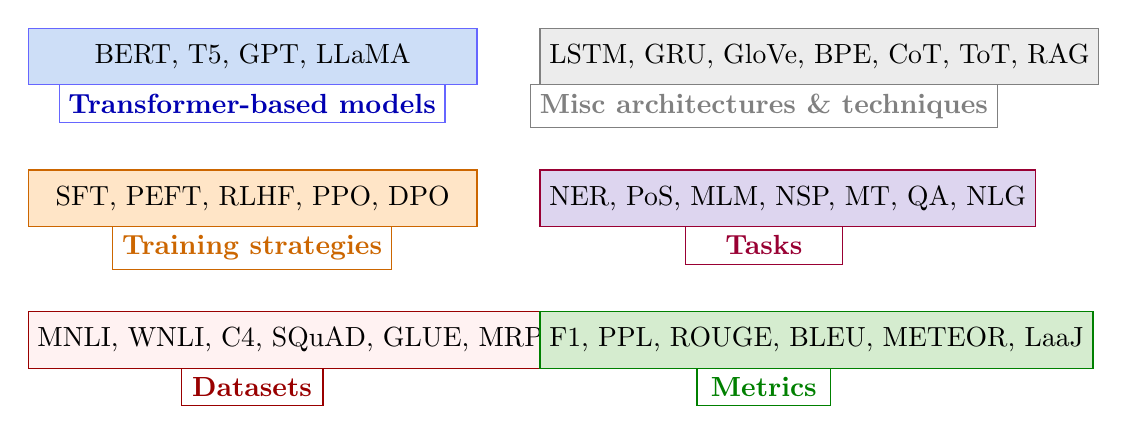
\begin{tikzpicture}[x=1cm,y=1cm]
  \node[draw=blue!60,fill=boxblue,minimum width=5.7cm,minimum height=0.72cm,anchor=west] at (0.0,5.0) {BERT, T5, GPT, LLaMA};
  \node[draw=blue!60,fill=white,anchor=north,font=\bfseries,text=blue!70!black,minimum width=3.7cm] at (2.85,4.65) {Transformer-based models};

  \node[draw=gray,fill=lightgray,minimum width=5.7cm,minimum height=0.72cm,anchor=west] at (6.5,5.0) {LSTM, GRU, GloVe, BPE, CoT, ToT, RAG};
  \node[draw=gray,fill=white,anchor=north,font=\bfseries,text=gray,minimum width=4.5cm] at (9.35,4.65) {Misc architectures \& techniques};

  \node[draw=orange!80!black,fill=boxorange,minimum width=5.7cm,minimum height=0.72cm,anchor=west] at (0.0,3.2) {SFT, PEFT, RLHF, PPO, DPO};
  \node[draw=orange!80!black,fill=white,anchor=north,font=\bfseries,text=orange!80!black,minimum width=3.0cm] at (2.85,2.85) {Training strategies};

  \node[draw=purple!80!black,fill=boxpurple,minimum width=5.7cm,minimum height=0.72cm,anchor=west] at (6.5,3.2) {NER, PoS, MLM, NSP, MT, QA, NLG};
  \node[draw=purple!80!black,fill=white,anchor=north,font=\bfseries,text=purple!80!black,minimum width=2.0cm] at (9.35,2.85) {Tasks};

  \node[draw=red!60!black,fill=pink!20,minimum width=5.7cm,minimum height=0.72cm,anchor=west] at (0.0,1.4) {MNLI, WNLI, C4, SQuAD, GLUE, MRPC};
  \node[draw=red!60!black,fill=white,anchor=north,font=\bfseries,text=red!60!black,minimum width=1.8cm] at (2.85,1.05) {Datasets};

  \node[draw=green!50!black,fill=boxgreen,minimum width=5.7cm,minimum height=0.72cm,anchor=west] at (6.5,1.4) {F1, PPL, ROUGE, BLEU, METEOR, LaaJ};
  \node[draw=green!50!black,fill=white,anchor=north,font=\bfseries,text=green!50!black,minimum width=1.7cm] at (9.35,1.05) {Metrics};
\end{tikzpicture}
\end{hitframe}

% ---------------------------------------------------------
\CourseOverview{1}

% ---------------------------------------------------------
\begin{hitframe}{NLP tasks overview}
\vspace{0.4cm}
\begin{tikzpicture}[x=1cm,y=1cm]
% Classification
\node[font=\Large\bfseries,anchor=west] at (0.3,5.0) {Classification};
\node[font=\ttfamily\small] (in1) at (0.7,4.2) {Input text};
\modelbox[right=0.25cm of in1] (m1) {Model};
\node[circle,draw,minimum size=0.50cm,right=0.25cm of m1] (out1) {3};
\draw[-{Latex[length=2mm]}] (in1) -- (m1);
\draw[-{Latex[length=2mm]}] (m1) -- (out1);
\node[anchor=west,align=left,font=\large] at (0.2,3.0) {$\bullet$ Sentiment extraction\\[2mm]$\bullet$ Intent detection\\[2mm]$\bullet$ Language detection\\[2mm]$\bullet$ Topic modeling};

% Multi-classification
\node[font=\Large\bfseries,anchor=west] at (4.7,5.0) {``Multi''-classification};
\node[font=\ttfamily\small] (in2) at (5.0,4.2) {Input text};
\modelbox[right=0.25cm of in2] (m2) {Model};
\node[font=\ttfamily\small,right=0.25cm of m2] (out2) {Input text};
\draw[-{Latex[length=2mm]}] (in2) -- (m2);
\draw[-{Latex[length=2mm]}] (m2) -- (out2);
\node[circle,draw,minimum size=0.44cm] at ([xshift=-0.15cm,yshift=-0.45cm]out2.south) {5};
\node[circle,draw,minimum size=0.44cm] at ([xshift=0.55cm,yshift=-0.45cm]out2.south) {1};
\node[anchor=west,align=left,font=\large] at (4.6,3.0) {$\bullet$ Part of speech tagging\\[2mm]$\bullet$ Named entity recognition\\[2mm]$\bullet$ Dependency parsing\\[2mm]$\bullet$ Constituency parsing};

% Generation
\node[font=\Large\bfseries,anchor=west] at (9.0,5.0) {Generation};
\node[font=\ttfamily\small] (in3) at (9.4,4.2) {Input text};
\modelbox[right=0.25cm of in3] (m3) {Model};
\node[font=\ttfamily\small,right=0.25cm of m3] (out3) {Out text};
\draw[-{Latex[length=2mm]}] (in3) -- (m3);
\draw[-{Latex[length=2mm]}] (m3) -- (out3);
\node[anchor=west,align=left,font=\large] at (8.9,3.0) {$\bullet$ Machine translation\\[2mm]$\bullet$ Question answering\\[2mm]$\bullet$ Summarization\\[2mm]$\bullet$ Text generation};
\end{tikzpicture}
\end{hitframe}

% ---------------------------------------------------------
\begin{hitframe}{NLP task: Sentiment Extraction}
\vspace{0.8cm}
\begin{center}
\begin{tikzpicture}[x=1cm,y=1cm]
\node[font=\ttfamily\large] (txt) at (3.0,4.2) {This teddy bear is SO CUTE!};
\modelbox[right=0.5cm of txt] (m) {Model};
\node[circle,draw,fill=boxgreen,minimum size=0.6cm,right=0.45cm of m] (plus) {+};
\draw[-{Latex[length=2.2mm]}] (txt) -- (m);
\draw[-{Latex[length=2.2mm]}] (m) -- (plus);
\node[anchor=west,font=\Large\bfseries] at (-1.2,2.7) {Datasets};
\node[anchor=west,font=\large] at (-0.7,2.1) {Amazon reviews};
\node[anchor=west,font=\large] at (4.5,2.1) {IMDB critiques};
\node[anchor=west,font=\large] at (9.2,2.1) {Twitter};
\node[anchor=west,font=\Large\bfseries] at (-1.2,1.25) {Evaluation metrics};
\node[anchor=west,align=left,font=\large] at (-0.8,0.55) {$\bullet$ Accuracy $\rightarrow$ \% of observations correctly predicted?\\[1.5mm]
$\bullet$ Precision $\rightarrow$ \% of predicted positive that were correct?\\[1.5mm]
$\bullet$ Recall $\rightarrow$ \% of actually positive that were correct?\\[1.5mm]
$\bullet$ F1 score $\rightarrow$ function of precision and recall};
\end{tikzpicture}
\end{center}
\end{hitframe}

% ---------------------------------------------------------
\CourseOverview{2}

% ---------------------------------------------------------
\begin{hitframe}{Tokenization}
\begin{center}
\vspace{0.65cm}
{\ttfamily\fontsize{22}{26}\selectfont A cute teddy bear is reading.}
\vspace{0.9cm}

\begin{tikzpicture}[x=1cm,y=1cm]
\node[anchor=east,font=\bfseries] at (0,2.3) {word};
\foreach \w/\x/\wd in {A/1/0.65,cute/2.1/1.0,teddy/3.55/1.15,bear/5.0/1.05,is/6.25/0.85,reading/7.65/1.35,./9.0/0.65}{
  \node[draw,minimum width=\wd cm,minimum height=0.55cm,font=\ttfamily] at (\x,2.3) {\w};
}
\node[anchor=east,font=\bfseries] at (0,1.15) {sub-word};
\foreach \w/\x/\wd in {A/1/0.65,cute/2.1/1.0,ted/3.25/0.70,\#\#dy/4.05/0.85,bear/5.05/1.05,is/6.25/0.85,read/7.35/1.0,\#\#ing/8.45/1.0,./9.35/0.55}{
  \node[draw,minimum width=\wd cm,minimum height=0.55cm,font=\ttfamily] at (\x,1.15) {\w};
}
\node[anchor=east,font=\bfseries] at (0,0.0) {character};
\foreach \w [count=\i] in {A,\_,c,u,t,e,\_,t,e,d,d,y,\_,b,e,a,r,\_,i,s,\_,r,e,a,d,i,n,g,.}{
  \node[draw,minimum width=0.35cm,minimum height=0.43cm,font=\ttfamily\scriptsize] at ({0.45+0.38*\i},0) {\w};
}
\end{tikzpicture}
\end{center}
\end{hitframe}

% ---------------------------------------------------------
\begin{hitframe}{Tokenization summary}
\vspace{0.35cm}
\renewcommand{\arraystretch}{1.55}
\begin{center}
\begin{tabular}{|>{\centering\arraybackslash}p{3.0cm}|p{4.8cm}|p{5.0cm}|}
\hline
\rowcolor{lightgray}\textbf{Method} & \centering\textbf{Pros} & \centering\arraybackslash\textbf{Cons} \\
\hline
\textbf{Word-level} &
$\bullet$ Simple\\ $\bullet$ Interpretable &
$\bullet$ Risk of OOV\\ $\bullet$ Does not leverage knowledge of root \\
\hline
\textbf{Subword-level}\\ e.g. WordPiece, BPE &
$\bullet$ Leverages common prefixes and suffixes\\ $\bullet$ Learned from the data &
$\bullet$ Risk of OOV, though less than word-level \\
\hline
\textbf{Character-level} &
$\bullet$ Small chance of OOV\\ $\bullet$ Robust to casing and misspellings &
$\bullet$ Makes computations slower\\ $\bullet$ Embeddings not interpretable \\
\hline
\end{tabular}
\end{center}
\end{hitframe}

% ---------------------------------------------------------
\CourseOverview{3}

% ---------------------------------------------------------
\begin{hitframe}{Token representations}
\vspace{0.25cm}
{\Large\bfseries Motivation}
\vspace{0.15cm}
\begin{center}
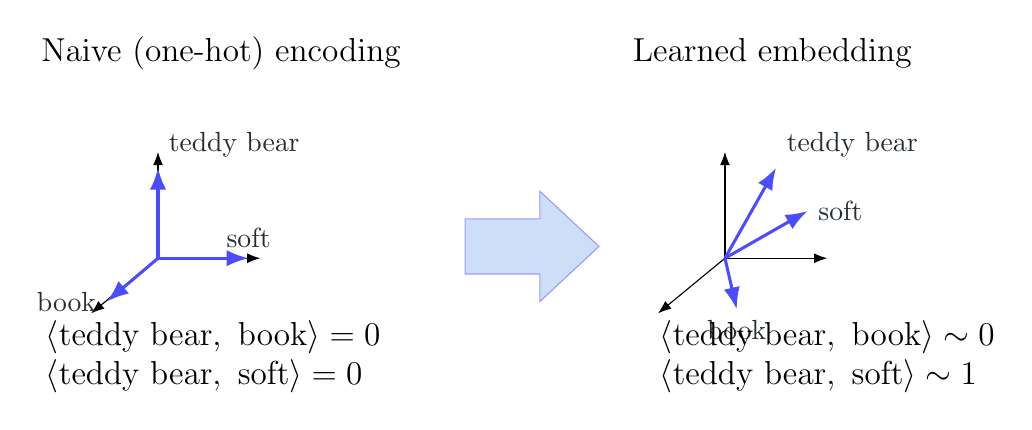
\begin{tikzpicture}[x=1cm,y=1cm]
% left axes
\node[font=\large] at (2.2,4.7) {Naive (one-hot) encoding};
\draw[-{Latex}] (1.4,2.1) -- (2.7,2.1);
\draw[-{Latex}] (1.4,2.1) -- (1.4,3.45);
\draw[-{Latex}] (1.4,2.1) -- (0.55,1.4);
\draw[blue!70,-{Latex},line width=1.1pt] (1.4,2.1) -- (1.4,3.25) node[above right,text=textdark] {teddy bear};
\draw[blue!70,-{Latex},line width=1.1pt] (1.4,2.1) -- (0.75,1.55) node[left,text=textdark] {book};
\draw[blue!70,-{Latex},line width=1.1pt] (1.4,2.1) -- (2.55,2.1) node[above,text=textdark] {soft};
\node[font=\large,align=left] at (2.1,0.85) {$\langle \text{teddy bear},\text{ book}\rangle=0$\\$\langle \text{teddy bear},\text{ soft}\rangle=0$};

% arrow
\draw[fill=boxblue,draw=blue!40] (5.3,2.6) -- (6.25,2.6) -- (6.25,2.95) -- (7.0,2.25) -- (6.25,1.55) -- (6.25,1.9) -- (5.3,1.9) -- cycle;

% right axes
\node[font=\large] at (9.2,4.7) {Learned embedding};
\draw[-{Latex}] (8.6,2.1) -- (9.9,2.1);
\draw[-{Latex}] (8.6,2.1) -- (8.6,3.45);
\draw[-{Latex}] (8.6,2.1) -- (7.75,1.4);
\draw[blue!70,-{Latex},line width=1.1pt] (8.6,2.1) -- (9.25,3.25) node[above right,text=textdark] {teddy bear};
\draw[blue!70,-{Latex},line width=1.1pt] (8.6,2.1) -- (8.75,1.45) node[below,text=textdark] {book};
\draw[blue!70,-{Latex},line width=1.1pt] (8.6,2.1) -- (9.65,2.7) node[right,text=textdark] {soft};
\node[font=\large,align=left] at (9.9,0.85) {$\langle \text{teddy bear},\text{ book}\rangle\sim 0$\\$\langle \text{teddy bear},\text{ soft}\rangle\sim 1$};
\end{tikzpicture}
\end{center}
\source{Figure style inspired by CS230/CME295 teaching material.}
\end{hitframe}

% ---------------------------------------------------------
\begin{hitframe}{Word2vec}
\vspace{0.35cm}
\textbf{Overview}
\begin{itemize}
  \item Neural network with a proxy task over billions of words worth of text
  \item Learns an embedding layer
\end{itemize}
\vspace{0.25cm}
\textbf{Proxy tasks}
\begin{itemize}
  \item CBOW: predict a word from its surrounding context
  \item Skip-gram: predict surrounding context from a center word
\end{itemize}
\vspace{0.25cm}
\begin{center}
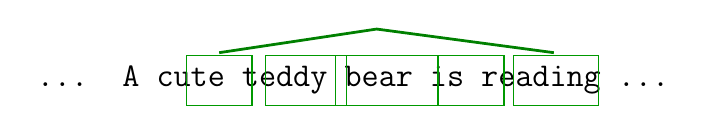
\begin{tikzpicture}[x=1cm,y=1cm]
\node[font=\ttfamily\large] at (4.0,1.1) {... A cute teddy bear is reading ...};
\node[draw=green!60!black,fit={(2.0,0.9) (2.6,1.3)}] {};
\node[draw=green!60!black,fit={(3.0,0.9) (3.8,1.3)}] {};
\node[draw=green!60!black,fit={(5.2,0.9) (5.8,1.3)}] {};
\node[draw=green!60!black,fit={(6.15,0.9) (7.0,1.3)}] {};
\draw[green!50!black,line width=1pt] (2.3,1.45) -- (4.3,1.75) -- (6.55,1.45);
\node[draw=green!60!black,fit={(3.9,0.9) (4.95,1.3)}] {};
\end{tikzpicture}
\end{center}
\source{Suggested reading: Mikolov et al. (2013), Efficient Estimation of Word Representations in Vector Space.}
\end{hitframe}

% ---------------------------------------------------------
\CourseOverview{4}

% ---------------------------------------------------------
\begin{hitframe}{Recurrent Neural Networks (RNNs)}
\vspace{0.35cm}
\textbf{Overview}
\begin{itemize}
  \item First introduced in the 1980s
  \item Class of neural networks where connections form a temporal sequence
\end{itemize}
\vspace{0.25cm}
\textbf{General form}
\vspace{0.1cm}
\begin{center}
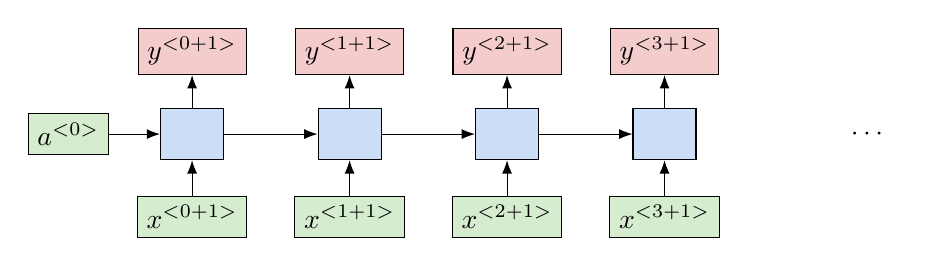
\begin{tikzpicture}[x=1cm,y=1cm]
\foreach \i/\txt in {0/A,1/cute,2/teddy bear,3/is}{
  \node[draw,fill=boxgreen,minimum width=0.8cm,minimum height=0.45cm] (x\i) at (1.4+2.0*\i,0.3) {$x^{<\i+1>}$};
  \node[draw,fill=boxblue,minimum width=0.8cm,minimum height=0.65cm] (h\i) at (1.4+2.0*\i,1.35) {};
  \node[draw,fill=boxpink,minimum width=0.8cm,minimum height=0.45cm] (y\i) at (1.4+2.0*\i,2.4) {$y^{<\i+1>}$};
  \draw[-{Latex}] (x\i) -- (h\i);
  \draw[-{Latex}] (h\i) -- (y\i);
}
\foreach \i in {0,1,2}{\draw[-{Latex}] (h\i) -- (h\the\numexpr\i+1\relax);}
\node[draw,fill=boxgreen,minimum width=0.8cm,minimum height=0.45cm,left=0.65cm of h0] (hinit) {$a^{<0>}$};
\draw[-{Latex}] (hinit) -- (h0);
\node at (10.0,1.35) {$\cdots$};
\end{tikzpicture}
\end{center}
\source{Figure style inspired by Stanford CS230 recurrent neural networks cheatsheet.}
\end{hitframe}

% ---------------------------------------------------------
\begin{hitframe}{Long Short-Term Memory (LSTM)}
\vspace{0.35cm}
\textbf{Overview}
\begin{itemize}
  \item Introduced in ``Long short-term memory'' (1997)
  \item Uses a more structured approach in the cell's hidden state
  \item Designed to mitigate vanishing gradients in long sequences
\end{itemize}
\vspace{0.25cm}
\textbf{General form}
\begin{center}
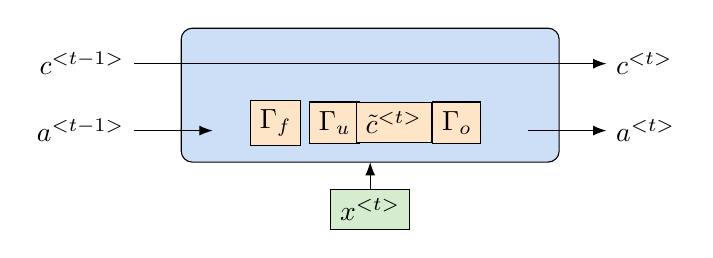
\begin{tikzpicture}[x=1cm,y=1cm]
  \node[draw,fill=boxblue,rounded corners,minimum width=4.8cm,minimum height=1.7cm] (cell) at (6,1.6) {};
  \draw[-{Latex}] (3.0,2.0) node[left] {$c^{<t-1>}$} -- (4.0,2.0) -- (8.0,2.0) -- (9.0,2.0) node[right] {$c^{<t>}$};
  \draw[-{Latex}] (3.0,1.15) node[left] {$a^{<t-1>}$} -- (4.0,1.15);
  \draw[-{Latex}] (8.0,1.15) -- (9.0,1.15) node[right] {$a^{<t>}$};
  \node[draw,fill=boxorange,minimum size=0.42cm] at (4.8,1.25) {$\Gamma_f$};
  \node[draw,fill=boxorange,minimum size=0.42cm] at (5.55,1.25) {$\Gamma_u$};
  \node[draw,fill=boxorange,minimum size=0.42cm] at (6.3,1.25) {$\tilde{c}^{<t>}$};
  \node[draw,fill=boxorange,minimum size=0.42cm] at (7.1,1.25) {$\Gamma_o$};
  \node[draw,fill=boxgreen,minimum width=0.8cm,minimum height=0.5cm] (x) at (6,0.15) {$x^{<t>}$};
  \draw[-{Latex}] (x) -- (6,0.75);
\end{tikzpicture}
\end{center}
\end{hitframe}

% ---------------------------------------------------------
\CourseOverview{5}

% ---------------------------------------------------------
\begin{hitframe}{History of attention}
\vspace{0.45cm}
\begin{itemize}
  \setlength\itemsep{0.25cm}
  \item Introduced in 2014 for neural machine translation
  \item Translation tasks had a real issue with long-term dependencies
  \item Seq2seq models struggled to ``remember'' the entire input sentence
\end{itemize}
\vspace{0.45cm}
\begin{center}
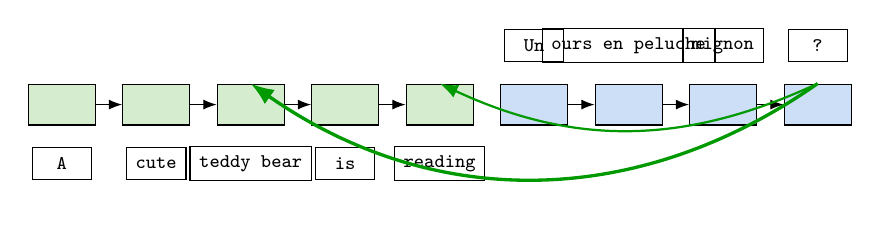
\begin{tikzpicture}[x=1cm,y=1cm]
\foreach \i/\w in {0/A,1/cute,2/teddy bear,3/is,4/reading}{
  \node[draw,fill=boxgreen,minimum width=0.85cm,minimum height=0.52cm] (enc\i) at (1.0+1.2*\i,1.1) {};
  \node[draw,minimum width=0.75cm,minimum height=0.4cm,font=\ttfamily\scriptsize] at (1.0+1.2*\i,0.35) {\w};
}
\foreach \i in {0,1,2,3}{\draw[-{Latex}] (enc\i) -- (enc\the\numexpr\i+1\relax);}
\foreach \i/\w in {0/Un,1/ours en peluche,2/mignon,3/?}{
  \node[draw,fill=boxblue,minimum width=0.85cm,minimum height=0.52cm] (dec\i) at (7.0+1.2*\i,1.1) {};
  \node[draw,minimum width=0.75cm,minimum height=0.4cm,font=\ttfamily\scriptsize] at (7.0+1.2*\i,1.85) {\w};
}
\foreach \i in {0,1,2}{\draw[-{Latex}] (dec\i) -- (dec\the\numexpr\i+1\relax);}
\draw[-{Latex},green!60!black,line width=1.2pt,bend left=35] (dec3.north) to (enc2.north);
\draw[-{Latex},green!60!black,line width=0.8pt,bend left=25] (dec3.north) to (enc4.north);
\end{tikzpicture}
\end{center}
\source{Suggested reading: Bahdanau et al. (2014), Neural Machine Translation by Jointly Learning to Align and Translate.}
\end{hitframe}

% ---------------------------------------------------------
\begin{hitframe}{Attention mechanism}
\vspace{0.35cm}
{\Large Concept of \textbf{Query}, \textbf{Key}, \textbf{Value}}
\vspace{1.0cm}
\begin{center}
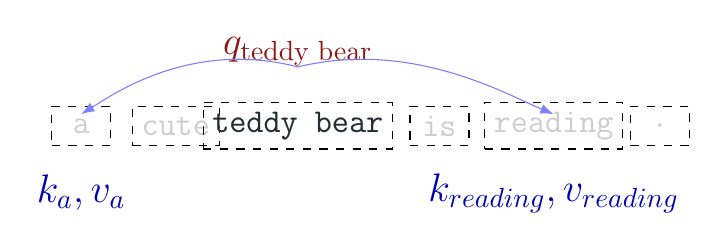
\begin{tikzpicture}[x=1cm,y=1cm]
\foreach \w/\x in {a/1,cute/2.2,teddy bear/3.75,is/5.55,reading/7.0,./8.35}{
  \node[draw,dashed,minimum height=0.5cm,minimum width=0.75cm,font=\ttfamily\large,text=fadegray] at (\x,0.0) {\w};
}
\node[draw,dashed,minimum width=1.9cm,minimum height=0.5cm,font=\ttfamily\large,text=textdark] at (3.75,0.0) {teddy bear};
\node[text=hitred,font=\Large] at (3.75,0.95) {$q_{\text{teddy bear}}$};
\node[text=blue!70!black,font=\Large] at (1.0,-0.85) {$k_a, v_a$};
\node[text=blue!70!black,font=\Large] at (7.0,-0.85) {$k_{reading}, v_{reading}$};
\draw[-{Latex},blue!50] (3.75,0.75) .. controls (2.4,1.1) and (1.4,0.4) .. (1.0,0.15);
\draw[-{Latex},blue!50] (3.75,0.75) .. controls (5.2,1.1) and (6.4,0.4) .. (7.0,0.15);
\end{tikzpicture}
\end{center}
\source{Inspired by the Query-Key-Value exposition in Super Study Guide / CME295.}
\end{hitframe}

% ---------------------------------------------------------
\begin{hitframe}{Attention mechanism}
\vspace{0.6cm}
\begin{center}
\Large Efficient computations with matrices:
\vspace{0.7cm}
\[
\mathrm{Attention}(Q,K,V)=
\mathrm{softmax}\left(\frac{QK^T}{\sqrt{d_k}}\right)V
\]
\vspace{0.5cm}
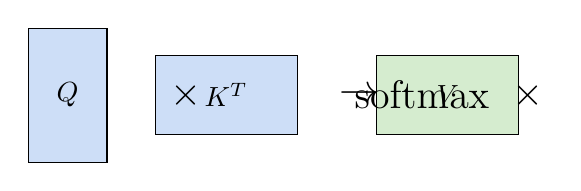
\begin{tikzpicture}[x=1cm,y=1cm]
\node[draw,fill=boxblue,minimum width=1.0cm,minimum height=1.7cm] (Q) at (2.5,0) {$Q$};
\node[draw,fill=boxblue,minimum width=1.8cm,minimum height=1.0cm,right=0.6cm of Q] (K) {$K^T$};
\node[draw,fill=boxgreen,minimum width=1.8cm,minimum height=1.0cm,right=1.0cm of K] (V) {$V$};
\node[font=\Large] at (4.0,0) {$\times$};
\node[font=\Large] at (6.2,0) {$\rightarrow$};
\node[font=\Large] at (7.0,0) {softmax};
\node[font=\Large] at (8.35,0) {$\times$};
\end{tikzpicture}
\end{center}
\end{hitframe}

% ---------------------------------------------------------
\CourseOverview{6}

% ---------------------------------------------------------
\begin{hitframe}{Overview of the Transformer}
\vspace{0.45cm}
\begin{itemize}
  \setlength\itemsep{0.25cm}
  \item Introduced in the 2017 paper \hlred{``Attention Is All You Need''}
  \item Relies on the \textbf{self-attention} mechanism
  \item Enabled highly parallel training and strong sequence modeling
\end{itemize}
\vspace{1.0cm}
\begin{center}
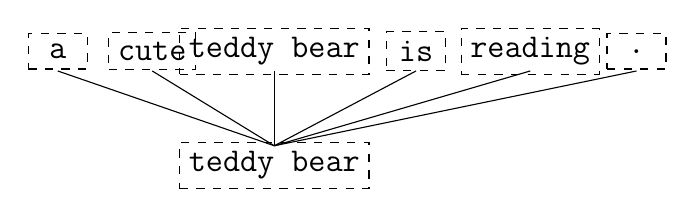
\begin{tikzpicture}[x=1cm,y=1cm]
\foreach \w/\x in {a/1,cute/2.2,teddy bear/3.75,is/5.55,reading/7.0,./8.35}{
  \node[draw,dashed,minimum height=0.45cm,minimum width=0.75cm,font=\ttfamily\large] (top\w) at (\x,0.7) {\w};
}
\node[draw,dashed,minimum width=1.9cm,minimum height=0.45cm,font=\ttfamily\large] (center) at (3.75,-0.75) {teddy bear};
\foreach \x in {1,2.2,3.75,5.55,7.0,8.35}{\draw (\x,0.45) -- (3.75,-0.5);}
\end{tikzpicture}
\end{center}
\source{Suggested reading: Vaswani et al. (2017), Attention Is All You Need.}
\end{hitframe}

% ---------------------------------------------------------
\begin{hitframe}{Transformer architecture}
\vspace{0.2cm}
\begin{columns}[T,onlytextwidth]
\column{0.42\textwidth}
\textbf{Encoder block}
\vspace{0.2cm}
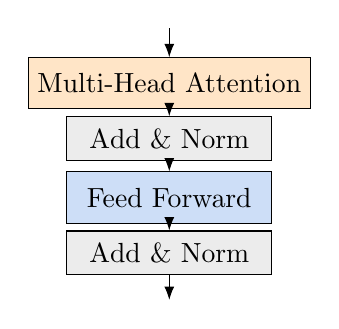
\begin{tikzpicture}[x=1cm,y=1cm]
\node[draw,fill=boxorange,minimum width=2.6cm,minimum height=0.65cm] (mha) at (2,2.9) {Multi-Head Attention};
\node[draw,fill=lightgray,minimum width=2.6cm,minimum height=0.55cm] (add1) at (2,2.2) {Add \& Norm};
\node[draw,fill=boxblue,minimum width=2.6cm,minimum height=0.65cm] (ffn) at (2,1.45) {Feed Forward};
\node[draw,fill=lightgray,minimum width=2.6cm,minimum height=0.55cm] (add2) at (2,0.75) {Add \& Norm};
\draw[-{Latex}] (2,3.6) -- (mha); \draw[-{Latex}] (mha) -- (add1); \draw[-{Latex}] (add1) -- (ffn); \draw[-{Latex}] (ffn) -- (add2); \draw[-{Latex}] (add2) -- (2,0.15);
\end{tikzpicture}

\column{0.56\textwidth}
\textbf{Main ingredients}
\begin{itemize}
  \setlength\itemsep{0.22cm}
  \item Token embeddings
  \item Positional information
  \item Multi-head self-attention
  \item Feed-forward network
  \item Residual connections
  \item Layer normalization
\end{itemize}
\end{columns}
\end{hitframe}

% ---------------------------------------------------------
\CourseOverview{7}

% ---------------------------------------------------------
\begin{hitframe}{End-to-end example}
\vspace{0.6cm}
\begin{center}
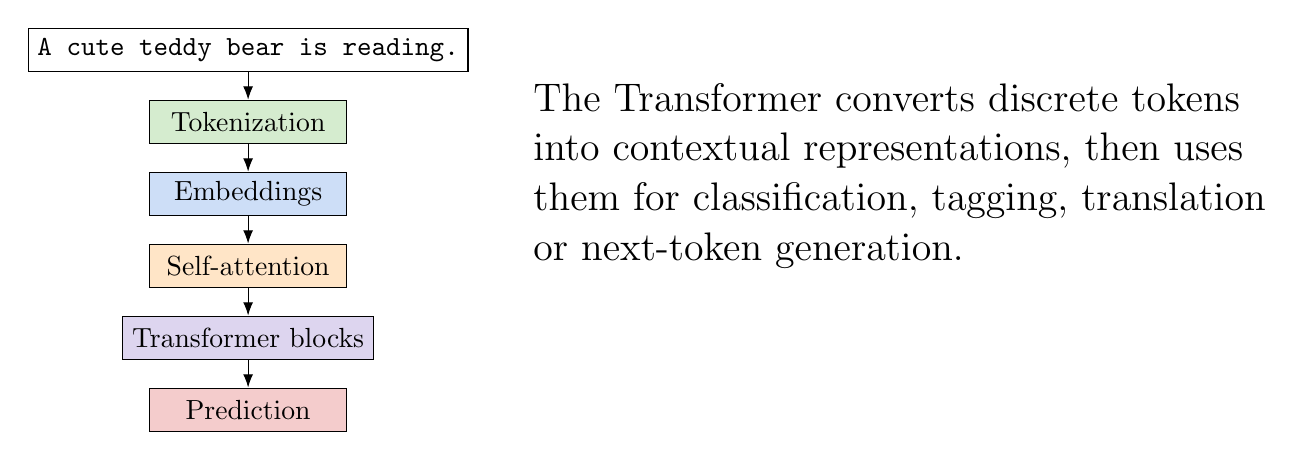
\begin{tikzpicture}[x=1cm,y=1cm,node distance=0.35cm]
\node[draw,minimum width=2.8cm,minimum height=0.55cm,font=\ttfamily] (text) at (1.5,3.6) {A cute teddy bear is reading.};
\node[draw,fill=boxgreen,minimum width=2.5cm,minimum height=0.55cm,below=of text] (tok) {Tokenization};
\node[draw,fill=boxblue,minimum width=2.5cm,minimum height=0.55cm,below=of tok] (emb) {Embeddings};
\node[draw,fill=boxorange,minimum width=2.5cm,minimum height=0.55cm,below=of emb] (att) {Self-attention};
\node[draw,fill=boxpurple,minimum width=2.5cm,minimum height=0.55cm,below=of att] (block) {Transformer blocks};
\node[draw,fill=boxpink,minimum width=2.5cm,minimum height=0.55cm,below=of block] (out) {Prediction};
\foreach \a/\b in {text/tok,tok/emb,emb/att,att/block,block/out}{\draw[-{Latex}] (\a) -- (\b);}
\node[anchor=west,align=left,font=\Large] at (5.0,2.0) {The Transformer converts discrete tokens\\into contextual representations, then uses\\them for classification, tagging, translation\\or next-token generation.};
\end{tikzpicture}
\end{center}
\end{hitframe}

% ---------------------------------------------------------
\begin{hitframe}{Key takeaways}
\vspace{0.55cm}
\begin{itemize}
  \setlength\itemsep{0.25cm}
  \item NLP contains classification, token-level prediction and generation tasks.
  \item Tokenization maps raw text to model-consumable units.
  \item Word2vec introduced useful dense word embeddings.
  \item RNNs and LSTMs model sequences, but are slow and struggle with long dependencies.
  \item Attention allows a model to dynamically focus on relevant tokens.
  \item Transformers replace recurrence with self-attention and scale extremely well.
\end{itemize}
\end{hitframe}

% ---------------------------------------------------------
\begin{hitframe}{Suggested reading}
\vspace{0.45cm}
\begin{itemize}
  \setlength\itemsep{0.25cm}
  \item Mikolov et al. (2013), \textit{Efficient Estimation of Word Representations in Vector Space}
  \item Hochreiter and Schmidhuber (1997), \textit{Long Short-Term Memory}
  \item Bahdanau et al. (2014), \textit{Neural Machine Translation by Jointly Learning to Align and Translate}
  \item Vaswani et al. (2017), \textit{Attention Is All You Need}
  \item Jurafsky and Martin, \textit{Speech and Language Processing}
\end{itemize}
\end{hitframe}

\begin{frame}[plain]
\begin{tikzpicture}[remember picture,overlay]
  \fill[white] (current page.south west) rectangle (current page.north east);
  \fill[hitred] (current page.north west) rectangle ([yshift=-0.72cm]current page.north east);
  \node[anchor=west,font=\fontsize{22}{26}\selectfont,text=white] at ([xshift=0.55cm,yshift=-0.36cm]current page.north west) {Questions?};
  \node[align=center,font=\fontsize{30}{36}\selectfont\bfseries,text=textdark] at (current page.center) {Questions?};
  \node[anchor=south west,font=\scriptsize\bfseries,text=textdark] at ([xshift=0.12cm,yshift=0.10cm]current page.south west) {Holon Institute of Technology};
  \node[anchor=south east,font=\scriptsize\bfseries,text=hitred] at ([xshift=-0.14cm,yshift=0.10cm]current page.south east) {HIT};
\end{tikzpicture}
\end{frame}

\end{document}
